\appendix

\pagebreak
\section{GitHub Repository README}

The following content is the README file taken from the FANS GitHub repository.

\def\pdffile{../../README.pdf}

\begin{center}
    \includegraphics[width=5in, page=1]{\pdffile}

    \includegraphics[width=5in, page=2]{\pdffile}

    \includegraphics[width=5in, page=3]{\pdffile}

    \includegraphics[width=5in, page=4]{\pdffile}

    \includegraphics[width=5in, page=5]{\pdffile}

    \includegraphics[width=5in, page=6]{\pdffile}

    \includegraphics[width=5in, page=7]{\pdffile}

    \includegraphics[width=5in, page=8]{\pdffile}
\end{center}

\section{Additional Use Cases} \label{ap:sequence}

The following sub-sections describe additional use cases that are handled by FANS, along with their sequence diagrams.

\subsubsection{Add New Contact Information Use Case}

This use case shown in Figure \ref{fig:add-contact} outlined the process wherein users added new contact information to
the FANS database. Through the web GUI, users entered new contact detail (phone numbers and email addresses) that
enabled the system to send emergency notifications. Upon submission, these details were successfully updated in the
real-time database. The message sequence diagram for this use case (not shown) illustrated the interactions between the
user, the web GUI, and the database, culminating in the notification system being updated with the new contact
information. This ensured that the FANS could reach the user through various channels in an emergency.

\begin{figure}
    \centering
    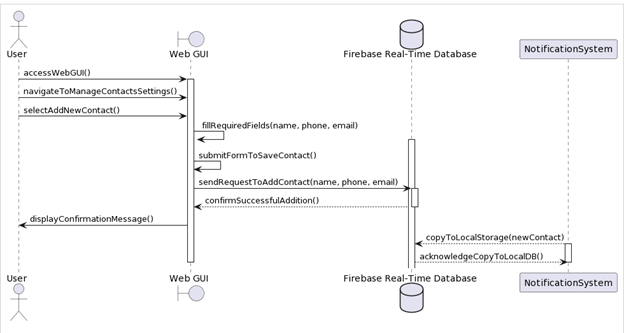
\includegraphics[width=\imagewidth]{../assets/sequence/AddingNewContactInformationSequenceDiagram.png}
    \caption{The sequence diagram for the adding new contact information use case.}
    \label{fig:add-contact}
\end{figure}
